\documentclass{beamer}
\usepackage[utf8]{inputenc}
\usepackage[serbian]{babel}
\usepackage{amsmath,amssymb,amsthm}
\usepackage{listings}
\usepackage{tikz}

\lstdefinelanguage{diff}{
	basicstyle=\ttfamily\small,
	morecomment=[f][\color{gray}]{@@},
	morecomment=[f][\color{green}]{+},
	morecomment=[f][\color{red}]{-},
}

\usefonttheme[onlymath]{serif}

\usetheme{Warsaw}

\title{Sistem za kontrolu verzija - Git}
\author{Du\v san Simi\' c}
\institute{%
	Departman za matematiku i informatiku \\
	Prirodno-matemati\v cki fakultet, Novi Sad \\
	Srbija
}
\date{7. jun 2022.}

\begin{document}

\begin{frame}
	\titlepage
\end{frame}

\begin{frame}
	\begin{itemize}
		\item \texttt{poslednja verzija.java}
		\item \texttt{poslednja finalna verzija.java}
		\item \texttt{poslednja finalna verzija2.java}
		\item \texttt{poslednja finalna verzija3.java}
		\item \texttt{poslednja finalna verzija3 kraj.java}
		\item \texttt{poslednja finalna verzija3 kraj zapravo.java}
	\end{itemize}
\end{frame}

\begin{frame}
	\begin{itemize}
		\item \texttt{dusan.tar.xz}
		\item \texttt{aca izmena.zip}
		\item \texttt{krsma izmena.zip}
		\item \texttt{finalna.tar.xz}
	\end{itemize}
\end{frame}

\begin{frame}{Sistemi za kontrolu verzija}
	\begin{itemize}
		\item Sistem za pra\' cenje izmena/revizija izvornog koda.
		\item Potreba za pra\' cenjem izmena tekstualnog sadr\v zaja.
		\item Obavezni deo razvoja softvera.
	\end{itemize}
\end{frame}

\begin{frame}{Git}
	\begin{columns}
		\column{0.5\textwidth}
		\begin{center}
			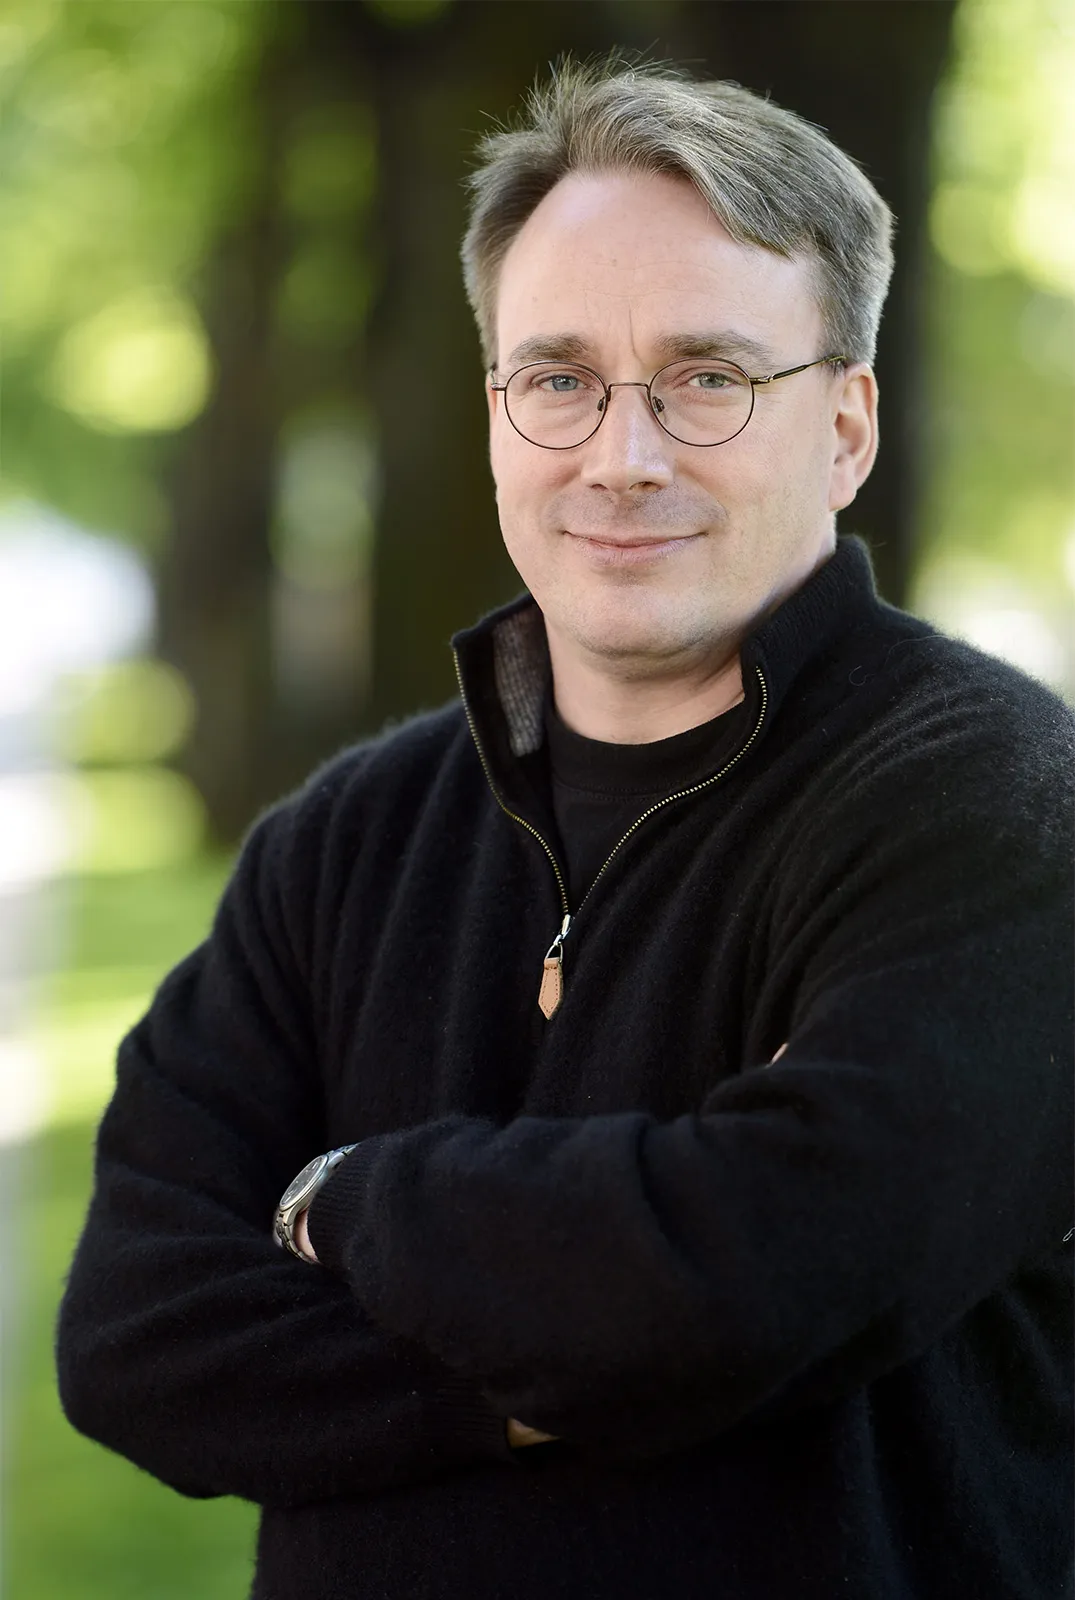
\includegraphics[scale=0.1]{torvalds.jpg}\\
			Linus Torvalds
		\end{center}
		\column{0.5\textwidth}
		\begin{center}
			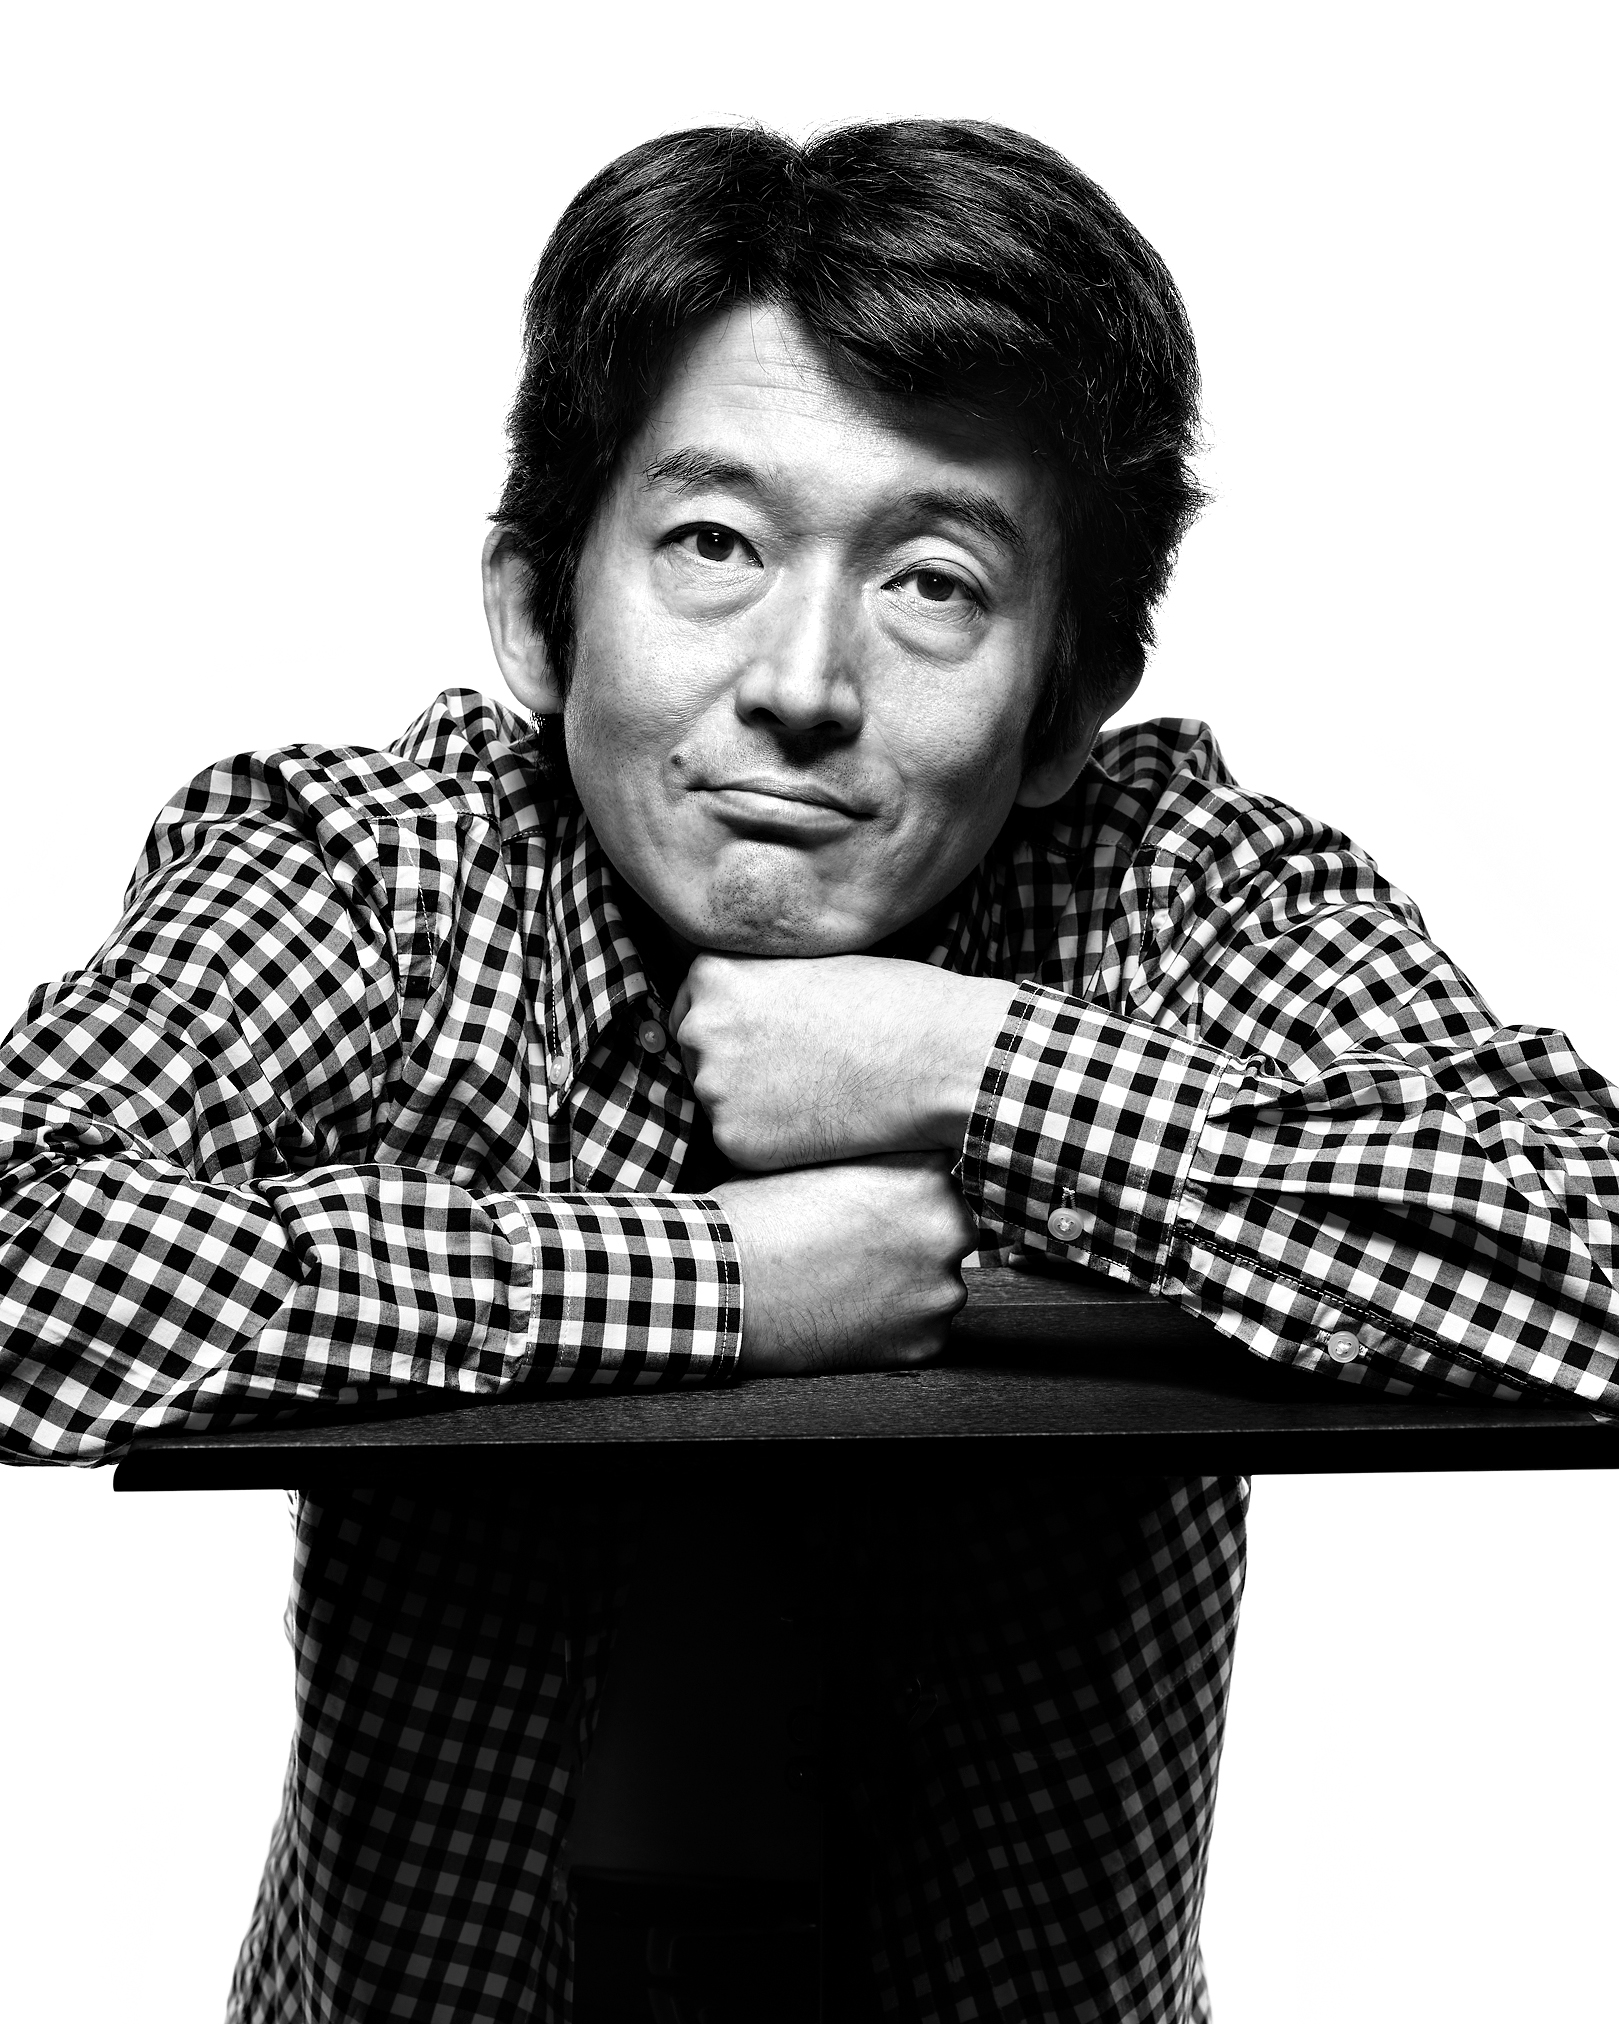
\includegraphics[scale=0.08]{hamano.jpg}\\
			Junio Hamano
		\end{center}
	\end{columns}
\end{frame}

\begin{frame}{Osnove git-a}
	\begin{itemize}
		\item Izmena/revizija (commit)
		      \pause
		\item Oznaka (tag)
		      \pause
		\item Glava (head)
		      \pause
		\item Grana (branch)
		      \pause
		\item Spajanje grana (merge commit)
		      \pause
		\item Tuma\v cenje razlika (diff)
	\end{itemize}
\end{frame}

\begin{frame}{Problem pra\' cenja izmena}
	Potrebno je pratiti izmene u tekstualnim (izvornim) datotekama,
	odmicanje razvoja, autora i vreme praveljanja tih izmena.

	\bigskip

	Tako\dj e je neophodno nedvosmisleno* identifikovanje svake izmene.
\end{frame}

\begin{frame}{Izmena/revizija (commit)}
	\begin{block}{Izmena/revizija (commit)}
		Svaka izmena se sastoji od izmenjenih linija u tekstualnim datotekama iz ugla korisnika, autora
		i datuma i vremena izmena kao i njenih najvi\v se dve a najmanje nijedna prethodna izmena.

		\begin{center}
			\begin{tikzpicture}[node distance={40pt}]
				\tikzstyle{c}=[circle]
				\tikzstyle{t}=[rectangle, fill=black!20]
				\tikzstyle{b1}=[fill=blue!20]

				\node[b1,c] (c1) {$c_1$};
				\node[b1,c] (c2) [right of=c1] {$c_2$};
				\node[b1,c] (c3) [right of=c2] {$c_3$};
				\node[b1,c] (c4) [right of=c3] {$c_4$};
				\node[b1,c] (c5) [right of=c4] {$c_5$};

				\foreach \from/\to in {c5/c4,c4/c3,c3/c2,c2/c1}
				\draw [->] (\from) -- (\to);
			\end{tikzpicture}
		\end{center}
	\end{block}

	\begin{block}{Identifikacija}
		Svaka izmena se identifikuje korist\' ci SHA-1 he\v s njenog sadr\v zaja.
	\end{block}
\end{frame}

\begin{frame}{He\v s funkcije i SHA-1}
	\begin{block}{He\v s funkcije}
		He\v s (eng. hash) funkcija je bilo koja funkcija koja slu\v zi za mapiranje podataka
		proizvoljne veli\v cine na vrednosti fiksne veli\v cine.
		\begin{align*}
			 & f \colon \textbf{d} \mapsto \textbf{h}, \textbf{d} \in [0, 255]_n \text{ gde je $ n $ prizvoljan broj}, \\
			 & \textbf{h} \in [0, 255]_m \text{ gde je $ m $ konstanta }
		\end{align*}
	\end{block}

	\begin{exampleblock}{SHA-1}
		Algoritam za he\v sovanje razvijen od strane Nacionalne sigurnosne agencije u Sjedinjenim
		Ameri\v ckim Dr\v zavama. Du\v zina izlaznog stringa je 160 bita ili 20 bajta ($ m = 20 $).
	\end{exampleblock}
\end{frame}

\begin{frame}{Oznaka (tag)}
	\begin{block}{Oznaka (tag)}
		Oznaka je string koji odgovara ta\v cno jednoj SHA-1 izlaznoj vrednosti (izmeni).

		\begin{center}
			\begin{tikzpicture}[node distance={40pt}]
				\tikzstyle{c}=[circle]
				\tikzstyle{t}=[rectangle, fill=black!20]
				\tikzstyle{b1}=[fill=blue!20]

				\node[b1,c] (c1) {$c_1$};
				\node[b1,c] (c2) [right of=c1] {$c_2$};
				\node[b1,c] (c3) [right of=c2] {$c_3$};
				\node[t] (v1) [above right of=c2] {1.0};
				\node[t] (v2beta) [above right of=c3] {2.0-beta};

				\foreach \from/\to in {c3/c2,c2/c1,v1/c2,v2beta/c3}
				\draw [->] (\from) -- (\to);
			\end{tikzpicture}
		\end{center}
	\end{block}

	\begin{exampleblock}{Primena}
		Verzije softvera, specijalne revizije\dots
	\end{exampleblock}
\end{frame}

\begin{frame}{Glava (head)}
	\begin{block}{Glava (head)}
		U git-u uvek ``gledate'' na neku odre\dj enu izmenu i ona je ozna\v cena tag-om ``HEAD''. Slu\v zi za
		informisanje korisnika gde se nalazi.

		\begin{center}
			\begin{tikzpicture}[node distance={40pt}]
				\tikzstyle{c}=[circle]
				\tikzstyle{t}=[rectangle, fill=black!20]
				\tikzstyle{b1}=[fill=blue!20]

				\node[b1,c] (c1) {$c_1$};
				\node[b1,c] (c2) [right of=c1] {$c_2$};
				\node[b1,c] (c3) [right of=c2] {$c_3$};
				\node[t] (HEAD) [above of=c2] {HEAD};

				\foreach \from/\to in {c3/c2,c2/c1,HEAD/c2}
				\draw [->] (\from) -- (\to);
			\end{tikzpicture}
		\end{center}
	\end{block}
\end{frame}

\begin{frame}{Grana (branch)}
	\begin{block}{Grana (branch)}
		Poslednja izmena u lancu bi trebala da ima posebnu vrstu oznake koja predstavlja naziv grane.
		Ukoliko nema oznake za granu, nije prakti\v cno pristupati toj grani.

		\begin{center}
			\begin{tikzpicture}[node distance={40pt}]
				\tikzstyle{c}=[circle]
				\tikzstyle{t}=[rectangle, fill=black!20]
				\tikzstyle{b1}=[fill=blue!20]
				\tikzstyle{b2}=[fill=red!20]

				\node[b1,c] (c1) {$c_1$};
				\node[b1,c] (c2) [right of=c1] {$c_2$};
				\node[b1,c] (c3) [right of=c2] {$c_3$};
				\node[b2,c] (c4) [above right of=c2] {$c_4$};
				\node[b2,c] (c5) [right of=c4] {$c_5$};
				\node[t] (feature) [right of=c5] {feature};
				\node[t] (main) [right of=c3] {main};

				\foreach \from/\to in {c3/c2,c2/c1,c5/c4,c4/c2,feature/c5,main/c3}
				\draw [->] (\from) -- (\to);
			\end{tikzpicture}
		\end{center}
	\end{block}

	\begin{exampleblock}{Primena}
		Neretko se nailazi u razvoju softvera na situaciju kada je potrebno da se vi\v se
		funkcionalnosti razvija paralelno ili da se paralelno razvijaju dve verzije softvera. Tu je
		idealno koristiti grane zbog lako\' ce pra\' cenja razvoja i kasnijeg dodavanja tih
		funkcionalnosti.
	\end{exampleblock}
\end{frame}

\begin{frame}{Grana (branch)}
	\begin{exampleblock}{Okle dokle ide grana}
		Postojanje grane je uvek relativno i zavisi od na\v cina na koji se gleda stablo.

		\begin{center}
			\begin{tikzpicture}[node distance={40pt}]
				\tikzstyle{c}=[circle]
				\tikzstyle{t}=[rectangle, fill=black!20]
				\tikzstyle{b1}=[fill=blue!20]
				\tikzstyle{b2}=[fill=red!20]
				\tikzstyle{b3}=[fill=green!20]

				\node[b1,c] (c1) {$c_1$};
				\node[b1,c] (c2) [right of=c1] {$c_2$};
				\node[b1,c] (c3) [right of=c2] {$c_3$};
				\node[b1,c] (c4) [right of=c3] {$c_4$};
				\node[b2,c] (c5) [below right of=c2] {$c_5$};
				\node[b2,c] (c6) [right of=c5] {$c_6$};
				\node[b3,c] (c7) [right of=c6] {$c_7$};
				\node[b3,c] (c8) [right of=c7] {$c_8$};
				\node[t] (feature1) [below right of=c6] {$\text{feature}_1$};
				\node[t] (feature2) [below right of=c8] {$\text{feature}_2$};
				\node[t] (main) [right of=c4] {main};

				\foreach \from/\to in {c8/c7,c7/c6,c6/c5,c5/c2,c4/c3,c3/c2,c2/c1,feature1/c6,feature2/c8,main/c4}
				\draw [->] (\from) -- (\to);
			\end{tikzpicture}
		\end{center}
	\end{exampleblock}
\end{frame}

\begin{frame}{Spajanje grana (merging)}
	\begin{columns}
		\column{0.5\textwidth}
		\begin{block}{Izmena spajanja (merge commit)}
			Izmena spajanja je ona koja ima dve izmene kao prethodnike.
		\end{block}

		\column{0.5\textwidth}
		\begin{center}
			\begin{tikzpicture}
				\tikzstyle{c}=[circle]
				\tikzstyle{b1}=[fill=blue!20]
				\tikzstyle{b2}=[fill=red!20]
				\tikzstyle{b3}=[fill=green!20]

				\node[b1,c] (c1) at (0, 0) {$c_1$};
				\node[b1,c] (c2) at (0, 2) {$c_2$};
				\node[b2,c] (c3) at (2, 0) {$c_3$};
				\node[b2,c] (c4) at (2, 2) {$c_4$};
				\node[b3,c] (m5) at (1, 4) {$m_5$};

				\foreach \from/\to in {m5/c4,m5/c2,c4/c3,c2/c1}
				\draw [->] (\from) -- (\to);
			\end{tikzpicture}
		\end{center}
	\end{columns}
\end{frame}

\begin{frame}
	\begin{center}
		\begin{tikzpicture}[node distance={40pt}]
			\tikzstyle{c}=[circle]
			\tikzstyle{t}=[rectangle, fill=black!20]
			\tikzstyle{b1}=[fill=blue!20]
			\tikzstyle{b2}=[fill=red!20]
			\tikzstyle{b3}=[fill=green!20]

			\node[b1,c] (c1) {$c_1$};
			\node[b1,c] (c2) [right of=c1] {$c_2$};
			\node[b1,c] (c3) [right of=c2] {$c_3$};
			\node[b1,c] (c4) [right of=c3] {$c_4$};
			\node[b1,c] (c5) [right of=c4] {$m_5$};
			\node[b1,c] (c6) [right of=c5] {$c_6$};
			\node[b2,c] (c7) [below of=c3] {$c_7$};
			\node[b2,c] (c8) [right of=c7] {$c_8$};
			\node[b3,c] (c9) [below of=c5] {$c_9$};
			\node[b3,c] (c10) [right of=c9] {$c_{10}$};
			\node[t] (head) [above right of=c6] {HEAD};
			\node[t] (main) [above left of=c6] {main};
			\node[t] (first) [below right of=c8] {first};
			\node[t] (second) [below right of=c10] {second};

			\foreach \from/\to in {c6/c5,c5/c4,c4/c3,c3/c2,c2/c1,c8/c7,c7/c2,c5/c8,c9/c8,c10/c9,head/c6,main/c6,first/c8,second/c10}
			\draw [->] (\from) -- (\to);
		\end{tikzpicture}
	\end{center}
\end{frame}

\begin{frame}[fragile]{Tuma\v cenje razlika (diff)}
	\begin{lstlisting}[language=diff, basicstyle=\tiny]
diff --git a/org.gtk.Gtk3theme.adw-gtk3.yaml b/org.gtk.Gtk3theme.adw-gtk3.yaml
index 45d2aaa..46dfb74 100644
--- a/org.gtk.Gtk3theme.adw-gtk3.yaml
+++ b/org.gtk.Gtk3theme.adw-gtk3.yaml
@@ -18,8 +18,8 @@ modules:
     sources:
       - type: archive
         strip-components: 0
-        url: https://github.com/lassekongo83/adw-gtk3/releases/download/v1.9/adw-gtk3v1-9.tar.xz
-        sha256: 293820f9e45e0ac4d730ec1dd753a6e06ebdfc2a7aababc72e7e21d3b6dae63d
+        url: https://github.com/lassekongo83/adw-gtk3/releases/download/v2.0/adw-gtk3v2-0.tar.xz
+        sha256: 57278d256730e7b026647ea6bc7bd2fb1a475f5765cd7618e2ddfa0d1c2631f0
 
   - name: appdata
     buildsystem: simple
\end{lstlisting}
\end{frame}

\begin{frame}
	\begin{center}
		\Huge Zaklju\v cak
	\end{center}
\end{frame}

\begin{frame}
	\begin{center}
		\Huge Pitanja
	\end{center}
\end{frame}

\end{document}
